% Gráfico: Ordenação - Nodes Left
\begin{figure}[htbp]
\centering
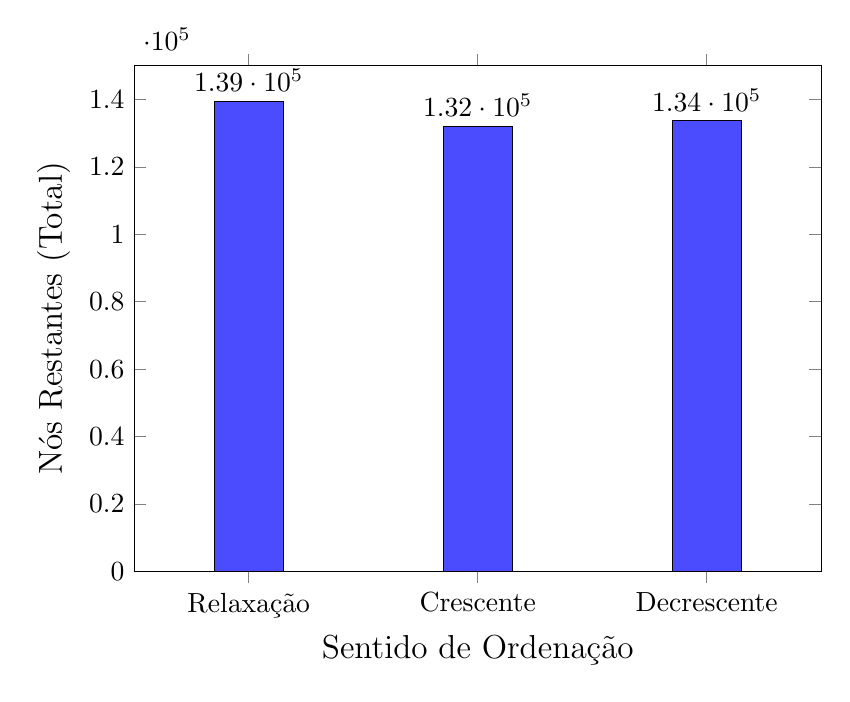
\begin{tikzpicture}
\begin{axis}[
    ybar,
    bar width=25pt,
    width=0.85\textwidth,
    height=8cm,
    ylabel={Nós Restantes (Total)},
    xlabel={Sentido de Ordenação},
    symbolic x coords={Relaxação, Crescente, Decrescente},
    xtick=data,
    nodes near coords,
    nodes near coords align={vertical},
    nodes near coords style={font=\normalsize},
    ymin=0,
    ymax=150000,
    enlarge x limits=0.25,
    ylabel style={font=\large},
    xlabel style={font=\large},
    tick label style={font=\normalsize},
]
\addplot[fill=blue!70] coordinates {
    (Relaxação,139460)
    (Crescente,131997)
    (Decrescente,133674)
};
\end{axis}
\end{tikzpicture}
\caption{Comparação do número total de nós restantes entre ordenação crescente e decrescente. A ordenação crescente (priorizando professores versáteis) obteve melhor desempenho com 131.997 nós restantes.}
\label{fig:nodes_order}
\end{figure}
